\section{Introducción}

Durante el cursado se desarrollaron los temas relacionados con el manejo de \emph{Verilog} y el flujo de diseño en Vivado 2024.2. Se propuso realizar el flujo completo sobre el proyecto de la figura \ref{fig:esq}. Este sistema consiste en un contador que enciende y apaga 4 leds a una frecuencia escogida por el usuario, haciendo uso de unos switches de entrada.

\begin{figure}[H]
    \centering
    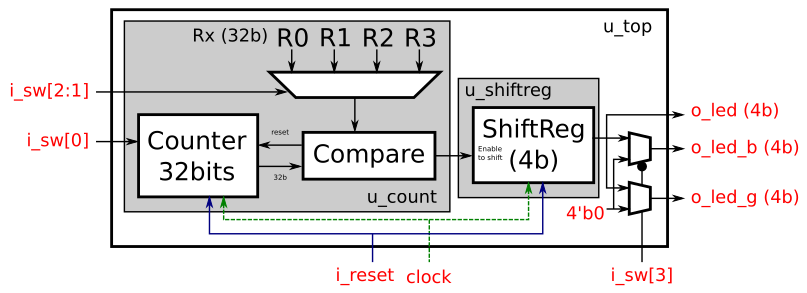
\includegraphics[width=0.85\linewidth]{img/esq.png}
    \caption{Esquema del diseño propuesto.}
    \label{fig:esq}
\end{figure}

Lo que realizan las interfaces es lo siguiente:

\begin{itemize}
    \item \texttt{o\_led}: es la salida hacia los leds blancos, presentes en la placa de evaluación.
    \item \texttt{o\_led\_b}: es la salida hacia los leds azules.
    \item \texttt{o\_led\_g}: es la salida hacia los leds verdes.
    \item \texttt{i\_sw[0]}: con esta entrada se controla el encendido del contador.
    \item \texttt{i\_sw[2:1]}: establecen el valor límite del contador.
    \item \texttt{i\_sw[3]}: enciende el led verde o azul.
    \item \texttt{i\_reset}: es un reset síncrono que establece el contador en cero y mantiene encendido el led en la primera posición.
\end{itemize}

\section{Desarrollo}

\subsection{Simulación}

Con el diseño en \emph{RTL} que se realizó en clase (anexo \ref{appx:rtl}) se desarrolló un testbench que prueba varios casos de entrada posible para observar si el módulo top responde correctamente. El código de este testbench también se encuentra en el anexo \ref{appx:rtl}.

Un aspecto a tener en cuenta es que, para la simulación se redujo la cantidad de bits del contador, para así poder apreciar las conmutaciones de los registros de salida con un menor tiempo de simulación.

Las formas de onda obtenidas se muestran en la figura \ref{fig:sim_graf}. En ellas se puede ver lo siguiente:

\begin{itemize}
    \item En la figura \ref{fig:sim_graf0} se observa que, sólo cuando \texttt{i\_switch[0]} vale \texttt{1} y el reset está levantado, los registros de \texttt{o\_led} cambian continuamente de valor, viéndose como si el \texttt{1} estuviera recorriendo estos registros.
    \item Al cambiar \texttt{i\_switch[2:1]}, cambia la velocidad en la que los registros de los leds se actualizan. Este efecto se puede ver en la figura \ref{fig:sim_graf3}.
    \item La figura \ref{fig:sim_graf5} muestra cómo el \texttt{i\_switch[0]} en 0 detiene la conmutación y el reset establece la posición del 1 de vuelta al principio del registro de leds.
\end{itemize}

\begin{figure}[t]
    \centering

    \begin{minipage}{\linewidth}
        \centering
        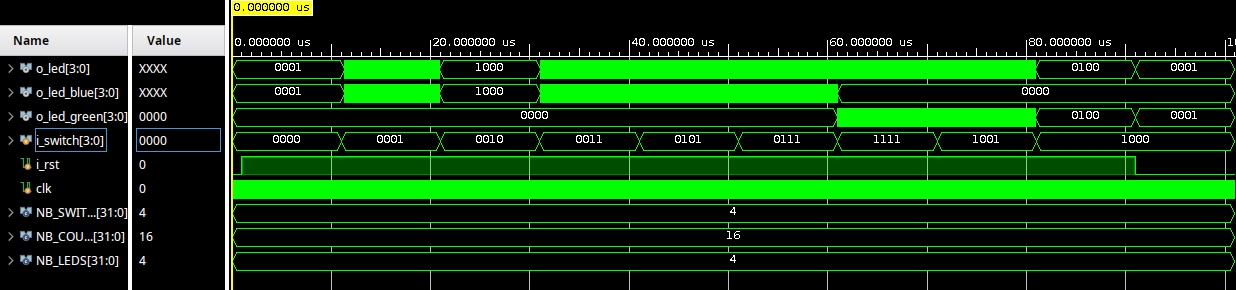
\includegraphics[width=1\linewidth]{img/sim_graf0.png}
        \subcaption{Toda la simulación.}
        \label{fig:sim_graf0}
    \end{minipage}
    
    \begin{minipage}{\linewidth}
        \centering
        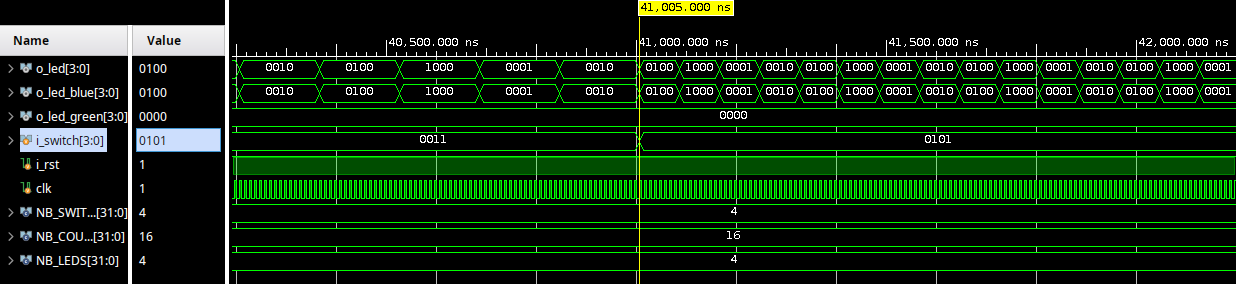
\includegraphics[width=1\linewidth]{img/sim_graf3.png}
        \subcaption{Cambio de velocidad en la conmutación de los leds.}
        \label{fig:sim_graf3}
    \end{minipage}
    
    \begin{minipage}{\linewidth}
        \centering
        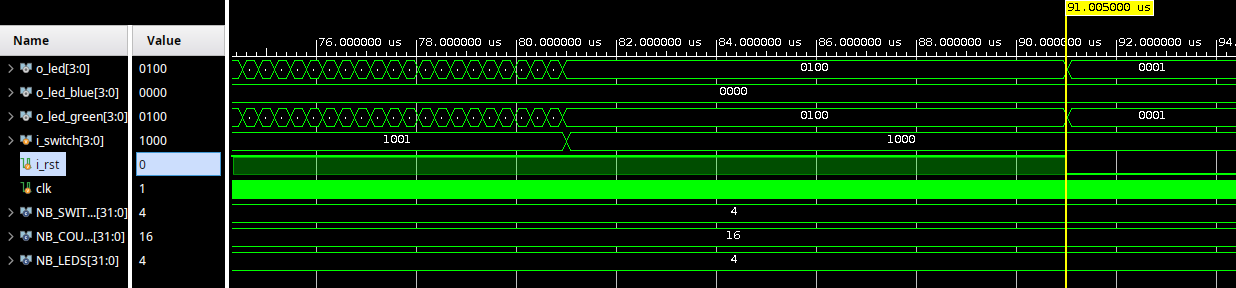
\includegraphics[width=1\linewidth]{img/sim_graf5.png}
        \subcaption{Deshabilitación y reset de la conmutación.}
        \label{fig:sim_graf5}
    \end{minipage}

    \caption{Formas de onda de la simulación.}
    \label{fig:sim_graf}
\end{figure}

\subsection{Implementación}

Luego de realizada la simulación, se implementó el diseño en la placa \emph{Arty A7} de \emph{Xilinx}, con el resultado mostrado en la figura \ref{fig:implementacion}. Como las FPGA disponibles para utilizar se deben controlar de forma remota, se implementó además dos IP cores en el diseño, provistas por la herramienta Vivado:

\begin{itemize}
    \item \emph{VIO}: Para controlar las entradas y observar las salidas sin necesidad de contar con la FPGA cerca.
    \item \emph{ILA}: Para observar la forma de onda de la salida.
\end{itemize}

\begin{figure}[H]
    \centering
    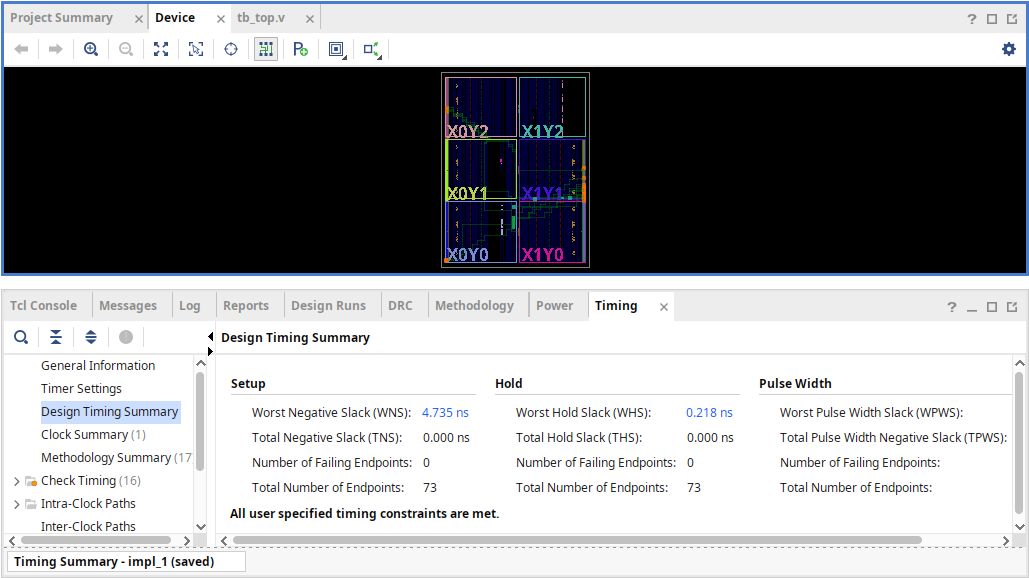
\includegraphics[width=0.8\linewidth]{img/implementacion.png}
    \caption{Captura de la implementación en Vivado.}
    \label{fig:implementacion}
\end{figure}

Las interfaces de estos bloques se muestra en la figura \ref{fig:bloques}. La entrada del ILA fue conectada a la interfaz \texttt{o\_led}, mientras que las entradas y salidas del VIO se conectaron de la siguiente forma:

\begin{itemize}
    \item \texttt{probe\_in0\_0}: \texttt{o\_led}
    \item \texttt{probe\_in1\_0}: \texttt{o\_led\_blue}
    \item \texttt{probe\_in2\_0}: \texttt{o\_led\_green}
    \item \texttt{probe\_out0\_0}: \texttt{select\_VIO}
    \item \texttt{probe\_out1\_0}: \texttt{reset\_from\_VIO}
    \item \texttt{probe\_out2\_0}: \texttt{switch\_from\_VIO}
\end{itemize}

Con estos dos IP, se realizó la implementación nuevamente, dando como resultado la pantalla de la figura \ref{fig:implementacion_vio_ila}.

\begin{figure}[H]
    \centering
    
    \begin{minipage}{0.56\linewidth}
        \centering
        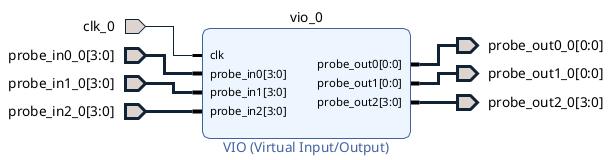
\includegraphics[width=\linewidth]{img/bloque_vio.png}
        \subcaption{Esquema del VIO.}
        \label{fig:bloque_vio}
    \end{minipage}
    \hfill
    \begin{minipage}{0.4\linewidth}
        \centering
        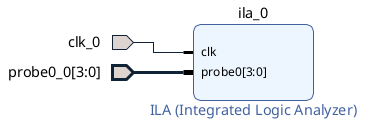
\includegraphics[width=\linewidth]{img/bloque_ila.png}
        \subcaption{Esquema del ILA.}
        \label{fig:bloque_ila}
    \end{minipage}

    \caption{Diagramas de los bloques IP utilizados en Vivado.}
    \label{fig:bloques}
\end{figure}

\begin{figure}[H]
    \centering
    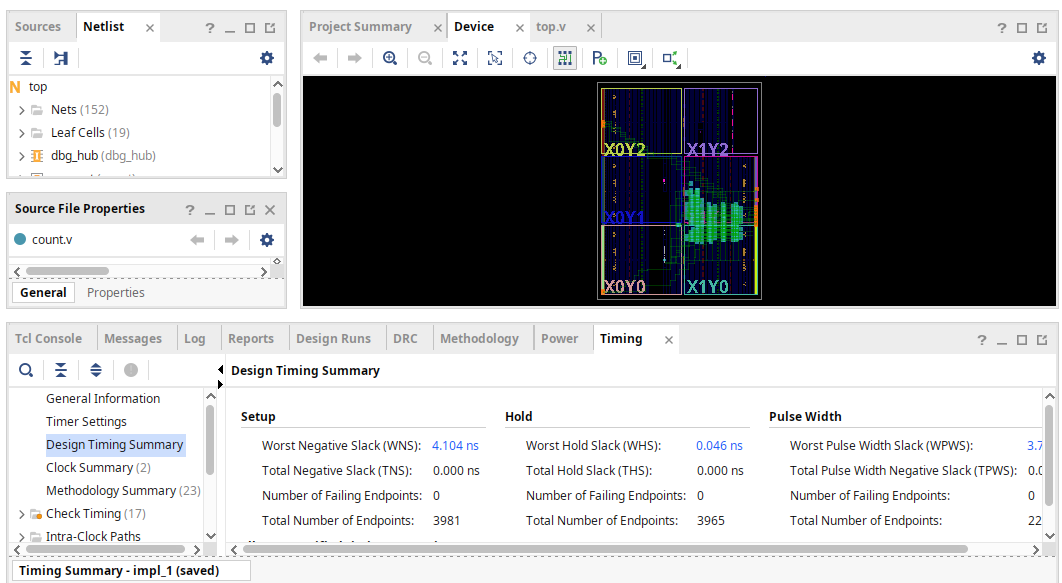
\includegraphics[width=0.8\linewidth]{img/implementacion_vio_ila.png}
    \caption{Captura de la implementación con VIO e ILA.}
    \label{fig:implementacion_vio_ila}
\end{figure}

\subsection{Control en una FPGA de Forma Remota}

Para conectarse en forma remota a una FPGA se abrió un túnel mediante \emph{SSH} al servidor donde se encuentran conectadas.

\begin{figure}[H]
    \centering
    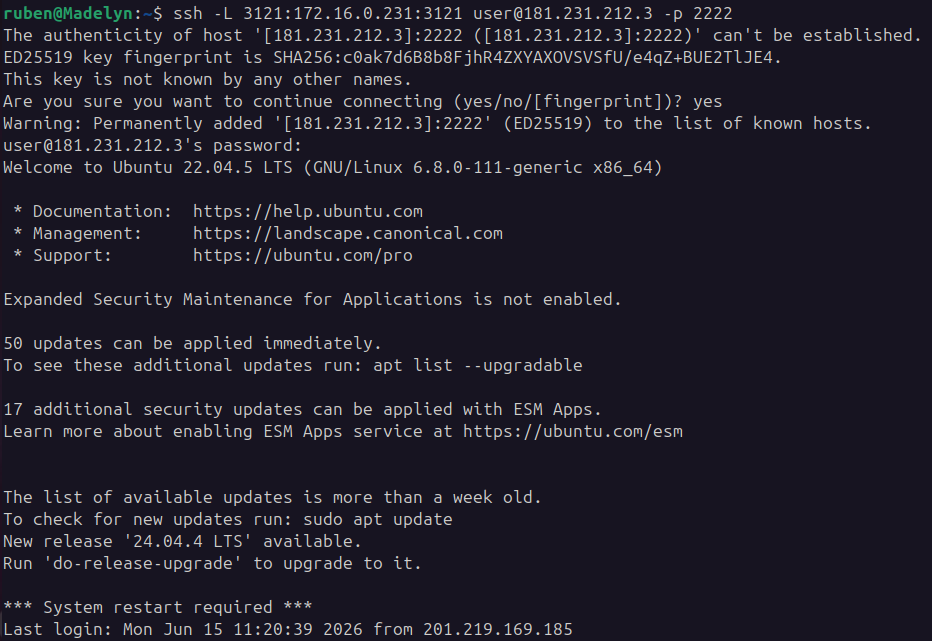
\includegraphics[width=0.85\linewidth]{img/tunel.png}
    \caption{Conexión por terminal al servidor de las FPGA.}
    \label{fig:tunel}
\end{figure}

Luego se entró al \emph{hardware manager} de Vivado, donde se seleccionó una de las FPGA disponibles y se le envió el bitstream del diseño; finalmente, se configuró el VIO y el ILA. La figura \ref{fig:botones} muestra la pantalla de control con el VIO. En este caso, el led azul (\texttt{probe\_in1}) es el que cambia, ya que el switch \texttt{probe\_out2[3]} está en 0. En la figura \ref{fig:otro_led} cambia el otro led cuando el switch está en 1.

\begin{figure}[H]
    \centering
    
    \begin{minipage}{0.48\linewidth}
        \centering
        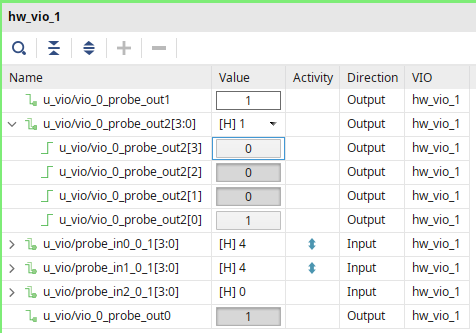
\includegraphics[width=\linewidth]{img/botones.png}
        \caption{Pantalla del VIO con la FPGA programada.}
        \label{fig:botones}
    \end{minipage}
    \hfill
    \begin{minipage}{0.48\linewidth}
        \centering
        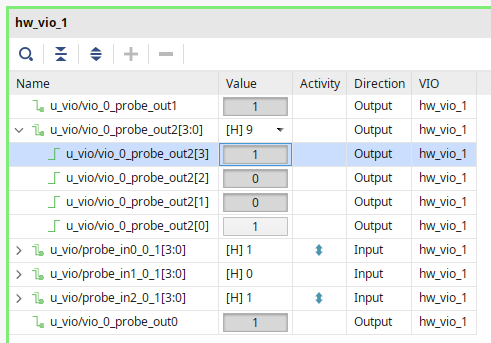
\includegraphics[width=\linewidth]{img/otro_led.png}
        \caption{Cambio de led en el VIO.}
        \label{fig:otro_led}
    \end{minipage}

\end{figure}

Para observar mejor la transición de los 1 en el ILA, se redujo el número de bits del contador de la misma manera que se redujo en la simulación. Con un valor de 12 bits, se obtuvieron las formas de onda de la figura \ref{fig:velocidad00}, \ref{fig:velocidad01}, \ref{fig:velocidad10} y \ref{fig:velocidad11}.

Finalmente, jugando con el trigger del ILA se puede observar el comienzo de la conmutación al levantar el reset, tal como se muestra en la figura \ref{fig:reset}.
    
\begin{figure}[H]
    \centering
    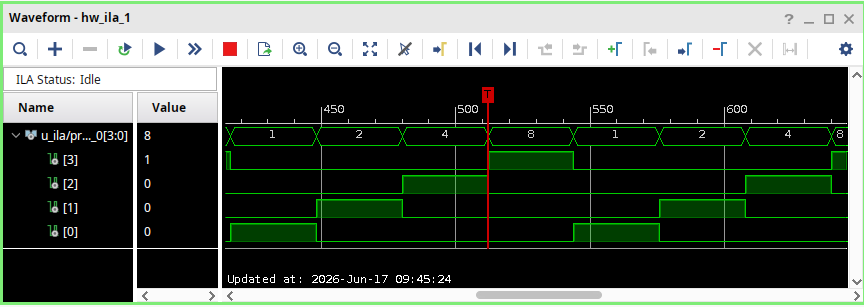
\includegraphics[width=0.9\linewidth]{img/velocidad00.png}
    \caption{Forma de onda en el ILA con \texttt{probe\_out2[2:1]=00}.}
    \label{fig:velocidad00}
\end{figure}
    
\begin{figure}[H]
    \centering
    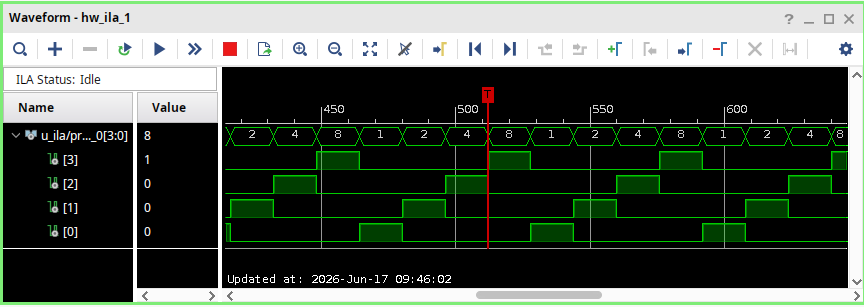
\includegraphics[width=0.9\linewidth]{img/velocidad01.png}
    \caption{Conmutación con \texttt{probe\_out2[2:1]=01}.}
    \label{fig:velocidad01}
\end{figure}

\begin{figure}[H]
    \centering
    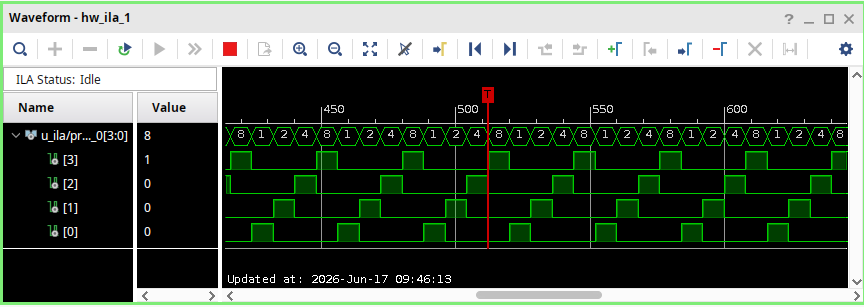
\includegraphics[width=0.9\linewidth]{img/velocidad10.png}
    \caption{Conmutación con \texttt{probe\_out2[2:1]=10}.}
    \label{fig:velocidad10}
\end{figure}

\begin{figure}[H]
    \centering
    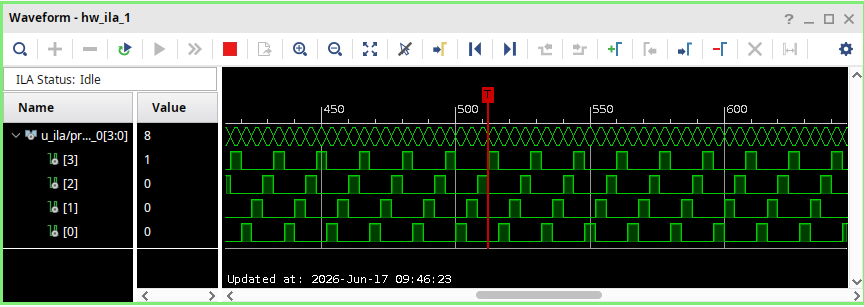
\includegraphics[width=0.9\linewidth]{img/velocidad11.png}
    \caption{Conmutación con \texttt{probe\_out2[2:1]=11}.}
    \label{fig:velocidad11}
\end{figure}

\begin{figure}[H]
    \centering
    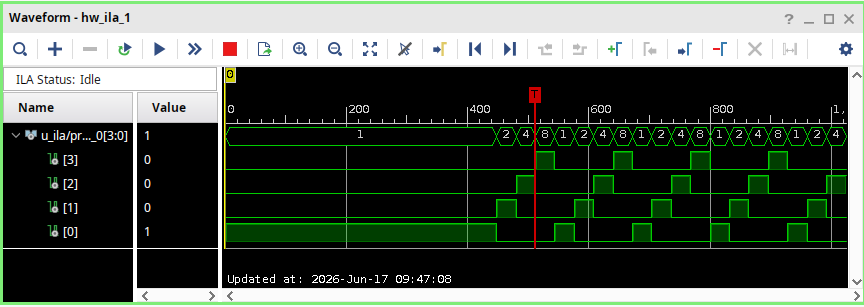
\includegraphics[width=0.9\linewidth]{img/reset.png}
    \caption{Comienzo de la conmutación al levantar el reset.}
    \label{fig:reset}
\end{figure}

\section{Conclusión}

Durante el desarrollo del RTL junto al testbench, se tuvo que tener en cuenta el factor de tiempo, ya que se fueron seleccionando iterativamente los valores límites del contador para poder observar la conmutación de los leds en la implementación. Por otro lado, se probaron varios casos de prueba en el testbench para garantizar que el funcionamiento sea el correcto; sin embargo, es posible introducir otros casos más al test, como por ejemplo, jugar con el switch mientras el reset está en 0.

\appendix

\section{Códigos en Verilog} \label{appx:rtl}

Los códigos en RTL y el testbench del proyecto se encuentran en el siguiente link: \url{https://github.com/Ruben-Zuniga/Introduccion-al-Disenio-Digital/tree/main/TP2}


% \[
%     V_{RRM} = V_{S12} = \sqrt{3} \ \hat{V}_{S} = \sqrt{3} \frac{\pi}{3\sqrt{3}} \ V_{L(AV)}
% \]

% \begin{equation}
%     \boxed{
%         V_{RRM} =  \frac{\pi}{3} \ V_{L(AV)}
%     }
% \end{equation}

% \begin{table}[H]
%     \centering
%     \begin{tblr}{
%         row{1} = {Titulo},
%         column{1} = {Titulo},
%         colspec = {Q[l] Q[c] Q[c]},
%         vlines,
%         hlines,
%         width=\linewidth
%     }
%         Parámetro & Símbolo & Valor \\
%         Máxima corriente de drenador continua ($T_C=25^\circ$C)                 & $I_{D,continua}$  & $36$ A            \\
%         Máxima tensión drenador-surtidor                                        & $V_{DSS}$         & $100$ V           \\
%         Resistencia drenador-surtidor en conducción ($V_{GS}=10$ V, $I_D=18$ A) & $R_{DS(on)}$      & $44$ m$\Omega$    \\
%         Máxima tensión puerta-surtidor                                          & $V_{GS}$          & $\pm 16$ V        \\
%         Tensión puerta-surtidor umbral                                          & $V_{GS(th)}$      & $1.4$ V           \\
%         Máxima disipación de potencia ($T_C=25^\circ$C)                         & $P_{max}$         & $140$ W           \\
%         Tiempo de retardo de encendido                                          & $t_{d(on)}$       & $11$ ns           \\
%         Tiempo de subida                                                        & $t_r$             & $81$ ns           \\
%         Tiempo de retardo de apagado                                            & $t_{d(off)}$      & $39$ ns           \\
%         Tiempo de bajada                                                        & $t_f$             & $62$ ns           \\

%     \end{tblr}
%     \caption{Parámetros característicos del IRL540.}
%     \label{tab:mosfet}
% \end{table}

% \begin{figure}[H]
%     \centering

%     \begin{minipage}{0.48\linewidth}
%         \centering
%         \includegraphics[width=1\linewidth]{img/ondas_completo1.png}
%     \end{minipage}
%     \hfill
%     \begin{minipage}{0.48\linewidth}
%         \centering
%         \includegraphics[width=1\linewidth]{img/ondas_completo2.png}
%     \end{minipage}

%     \caption{Formas de onda teóricas del convertidor.}
%     \label{fig:ondas}
% \end{figure}

% \begin{figure}[H]
%     \centering
%     \includegraphics[width=0.85\linewidth]{img/sim.png}
%     \caption{Formas de onda del rectificador hexafásico.}
%     \label{fig:sim}
% \end{figure}